\subsection{Positionsmessung}\label{Positionsmessung}
	Um Motoren genau Regeln zu k�nnen ist es meistens n�tig die Position des Rototrs zu messen. Dies kann wie folgt umgesetzt werden:

	\subsubsection{Back-EMF}
		Wenn in einer Spule sich der Stromfluss �ndert, wird eine Spannung induziert, im Fall von Synchronmaschinen wird diese Spannung Back-EMF genannt. Diese kann gemessen werden und es kann anhand dieser die Position und Drehzahl des Rotors ermittelt werden.
		
	\begin{figure}[H]
			\centering
			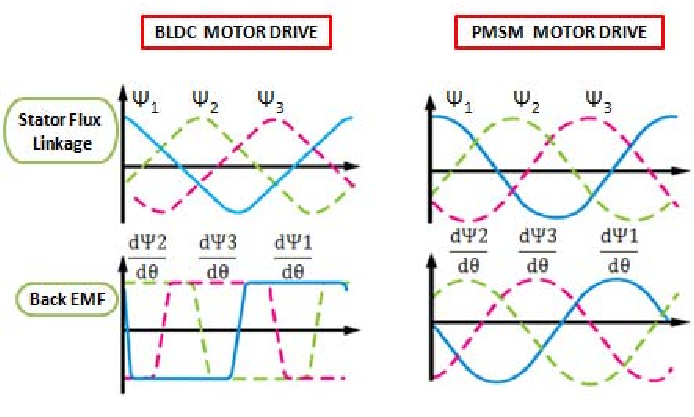
\includegraphics[scale=0.5]{./3_Stand_der_Technik/Abbildungen/PMSM_Back-EMF_1}
			\caption{Back-EMF Synchronmaschine\cite{Rode2023}}
	\end{figure}
	
	\subsubsection{Hall-Sensoren}
		Der Hall-Sensor ist ein magnetotastischer Sensor, er misst das magnetische Gleichfeld innerhalb eines Halbleiterpl�ttchens. Das Feld des Magneten durchsetzt das Pl�ttchen senkrecht, sodass die Ladungstr�ger aus ihrer Bahn abgelenkt werden. Es kann nun eine zum Feld proportionale Hall-Spannung abgegriffen werden.
		
		\begin{equation}
			U_{H} =  R_{H}*I*\frac{B}{d}
		\end{equation}
		
		$U_{H} \cdots$ Hallspannung \newline
		$R_{H} \cdots$ Hallkonstante \newline
		$I \cdots$ Pl�ttchenstrom \newline
		$B \cdots$ Induktion \newline
		$d \cdots$ Dicke des Pl�ttchens \newline
		
		Indem man 3 solcher Hall Sensoren hinter einem Motor anbringt kann so die Position und Drehzahl des Motors gemessen werden. Die Genauigkeit der Positionsmesung h�ngt dabei von der Anzahl der Polpaare ab. Desto mehr, desto genauer ist die Messung\cite{JulinHorstkoetter2023}
		
		\begin{figure}[H]
			\centering
			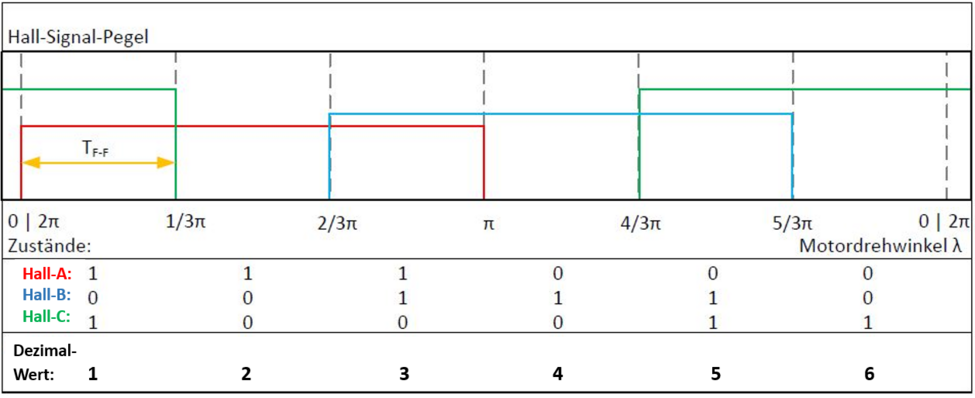
\includegraphics[scale=0.5]{./3_Stand_der_Technik/Abbildungen/Hall-Sensor_1}
			\caption{Ausgangssignal der Hallsensoren je nach Winkel des Rotors\cite{JulinHorstkoetter2023}}
		\end{figure}
	
	\subsubsection{Resolver / Drehgeber}
		Resolver oder Drehgeber sind beide Sensoren zur genauen Ermittlung der Motorposition. Die Genauigkeit h�ngt nur noch von der Bauweise des Sonsors ab und nicht von der des Motors. Sie k�nnen beide Inkremental oder Absolut den Winkel des Motors angeben. Der Unterschied zwischen beiden liegt darin, dass der Drehgeber ein digitales Signal ausgibt und der Resolver ein analoges.